1 - What is known

In the biosensor's community most findings and desicions in designed are achived 
through experimental analyses, trial and error procedures. Using
software to advice the design and manufacturing process can play a key role. In 
the world of plasmonics there are few softwares that are used to study Localized
Surface Plasmon Resonance. Among the most known softwares are COMSOL Multiphysics
a proprietary finite-element platform ({\color{red}cite COMSOL Multiphysics® v. 5.2. 
www.comsol.com. COMSOL AB, Stockholm, Sweden. NOT SURE HOW TO ADD THIS TO BIB} ), 
BEM++ ({\color{red}NOT SURE HOW TO CITE}) an open-source Boundary element method
library to solve time-harmonic Maxwell equations in 3D, and 
MNPBEM, an open-source Matlab toolbox for the simulation of metallic nanoparticles that
uses BEM and Hierarchical matrices \cite{Hohenester2018}. Besides, on the 
biosensing approach, the biomolecular electrostatic implementation of 
\pygbe \cite{CooperETal2016} allowed the study of ligand molecule orientation 
sensor \cite{CooperClementiBarba2015}.



2 - What is UNknown, limitations and gaps

Experiments suggests that the distance between the nanoparticle and the analyte 
affects the sensitivity of the sensor \cite{HaesETal2004}. 

Unkown: relation between high dependance on sensitivity on distance in LSPR biosensors.
Find structural details of analyte and nanoparticle, and the relative position between them.
Studies that deal with real protein geometry. 

Limitation: 
            - Software only study plasmonic assuming a non-lossy medium. 


limitations - BEM++ Chris any input in this, limitations?  
              private are expensive and not accessible, 
              matlab not free, 
              no grid convergence analysis or error study, 
              no reproducible framework 
              problem size, geometry, and computation time



Gap: study this using fast, free-software dependencies and open source computer
simulations. 





3 - Burning question, experimental approach, why ours is new and diff (fill the gap)

Solve this problem with pygbe? yes

long wavelength limit we don't need full Maxwell eq, we can approach it using
electrostatics.

\textit{Localized surface plasmon resonance} (LSPR) biosensor This type
of biosensors measure the shift of plasmon resonace frequency in metallic nanoparticles
when a target molecules binds to it. LSPR is an optical effect, but electrostatics 
makes a good approximation in the long-wavelength limit. In this work we use
PyGBe's approach to study how the LSPR response changes in the presence of a 
biomolecule.


\pygbe most recent 
application \cite{ClementiETal2017} tends to bridge that gap providing via
simulations, insights to guide the reasearch process. 

The latest release of \pygbe
extends the software to nanoplasmonics treating localized surface plasmon 
resonance (LSPR) quasi-statically \cite{MayergoyzZhang2007}.

Mentions that uses treecode, gmres and GPU. 

The software \footnote{\url{https://github.com/barbagroup/pygbe}} is shared 
under the BSD 3-clause license and the development repository is available on 
Github.












\begin{figure}[h] %  figure placement: here, top, bottom, or page
   \centering
   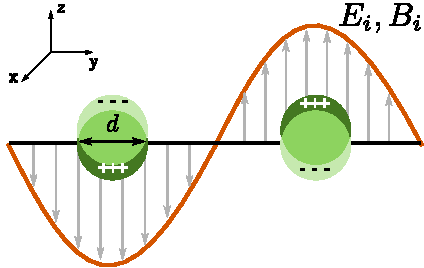
\includegraphics[width=0.35\textwidth]{lspr.pdf} 
   \caption{Localized Surface Plasmon Resonance (LSPR) scheme. LSPR is an 
            optical phenomenon that ocurrs when light shines on conductive 
            nanoparticles that are smaller than the wavelength of the incident 
            light. The free electrons on the surface of the nanoparticle are 
            excited by the incoming electric field oscillating with it and 
            creating plasmons}
   \label{fig:lspr}
\end{figure}




